\subsection{Leptonically decaying boson}
\label{subsec:leptons_selection}

Events are categorized into 0-, 1- and 2-lepton channels by number of Loose leptons in the final state. The common definition of Loose lepton (see Sec.~\ref{sec:ObjectDefinition}) ensures three channels to be orthogonal. 
Basically we can follow the event selections used in the previous analysis based on the 36\,\ifb dataset\cite{Ryzhov:2310214}.
This section focuses on the dedicated selection we have for the three leptons channels.

%%% 0-lepton channel


%%% 1-lepton channel
\clearpage
\subsubsection{1-lepton channel}
\label{subsubsec:1lep_event_selection}
This section summarizes the SR definitions in 1-lepton channel.

\textbf{$W \to \ell\nu$}

To select events consistent with $W \to \ell\nu$ candidate, exactly one Tight lepton is required. In addition,
the following cuts are defined for all regions as common cuts:

\begin{itemize}
\item $\met > 80 \,\GeV$
\item $\ptl > 28 \,\GeV$ %and \textcolor{red}{I think this is related to lepSF binning} 
%\item $m_{J} > 50 \, \GeV$ (merged only)
\end{itemize}
are applied in the merged (resolved) analysis to suppress the multi-jet background.
Merged and resolved regime selections are discussed in details in Section \ref{subsec:sr_selection}.

Examples of distributions for MC samples as well as observed data are shown in Figure \ref{fig:1LepPreselCuts}; in particular, we can nicely see the W-peak in the $t\bar{t}$ process.

%\textcolor{red}{do we have any d-phi selection in 1-lep?? NO , this comment can be deleted after}

\begin{figure}[ht]
\centering
        \begin{subfigure}{0.3\textwidth}
            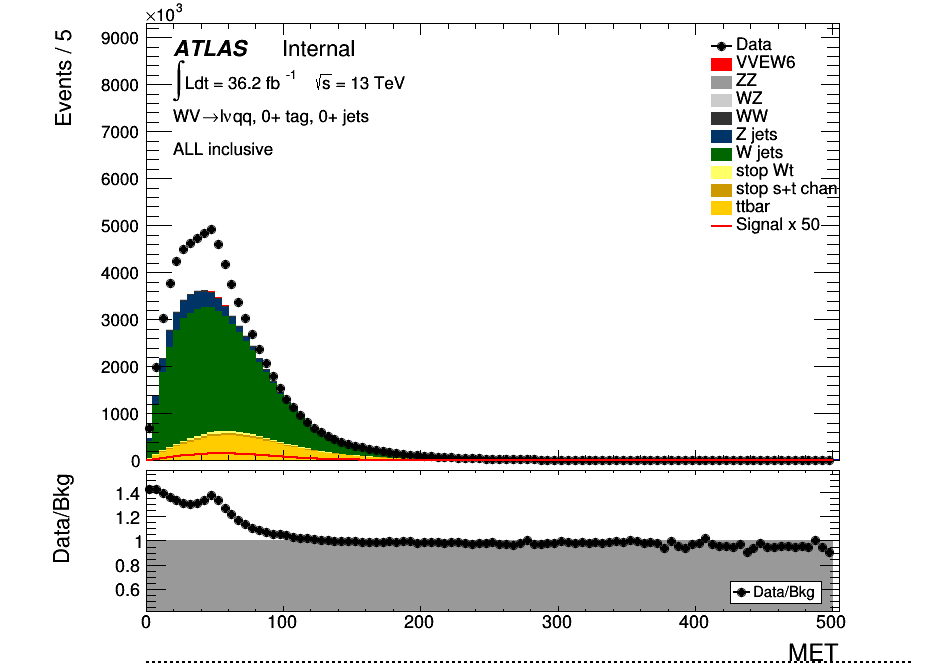
\includegraphics[width=\linewidth]{figures/1lep/CRPlots/C_0ptag0pjet_0ptv_ALL_MET_Lin.png}
            \caption{$E_{T,miss}$ before any event selection.}
        \end{subfigure}
        \begin{subfigure}{0.3\textwidth}
            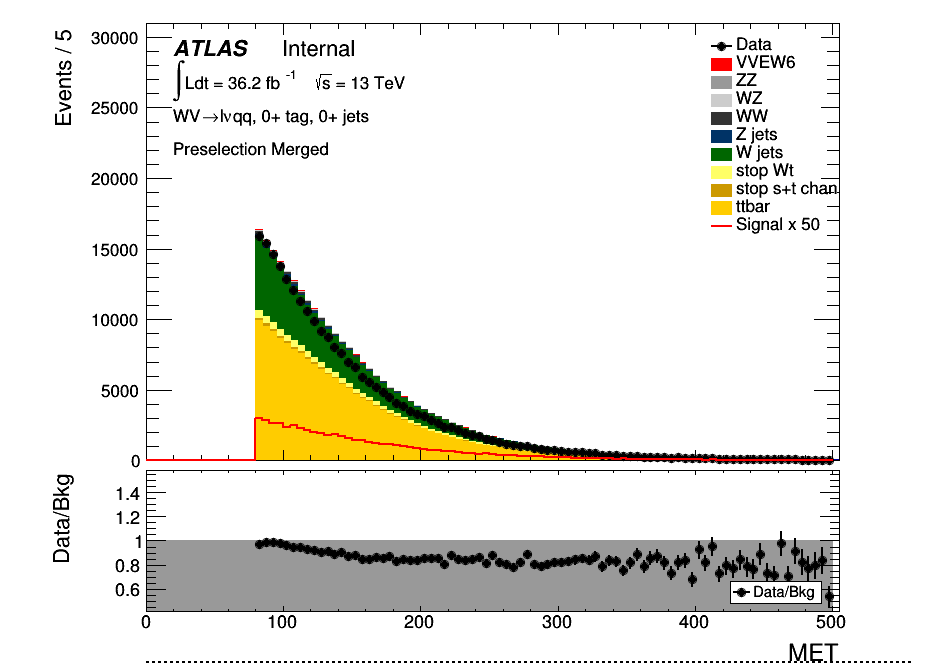
\includegraphics[width=\linewidth]{figures/1lep/CRPlots/C_0ptag0pjet_0ptv_Presel_Merged_MET_Lin.png}
            \caption{$E_{T,miss}$ after merged common preselection.}
        \end{subfigure}
        \begin{subfigure}{0.3\textwidth}
            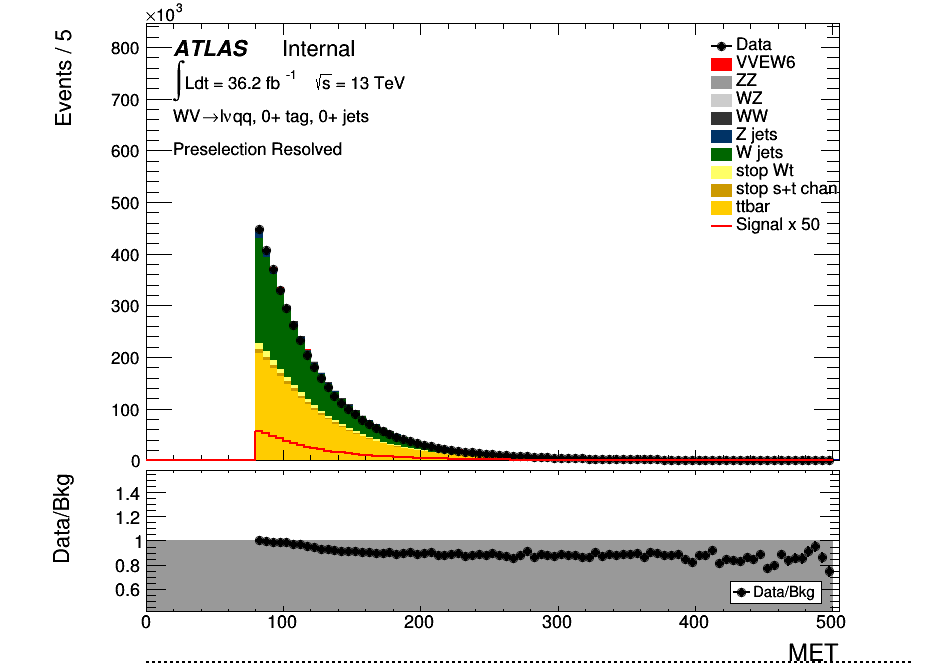
\includegraphics[width=\linewidth]{figures/1lep/CRPlots/C_0ptag0pjet_0ptv_Presel_Resolved_MET_Lin.png}
            \caption{$E_{T,miss}$ distribution after resolved common preselection.}
        \end{subfigure} \\

        \begin{subfigure}{0.3\textwidth}
            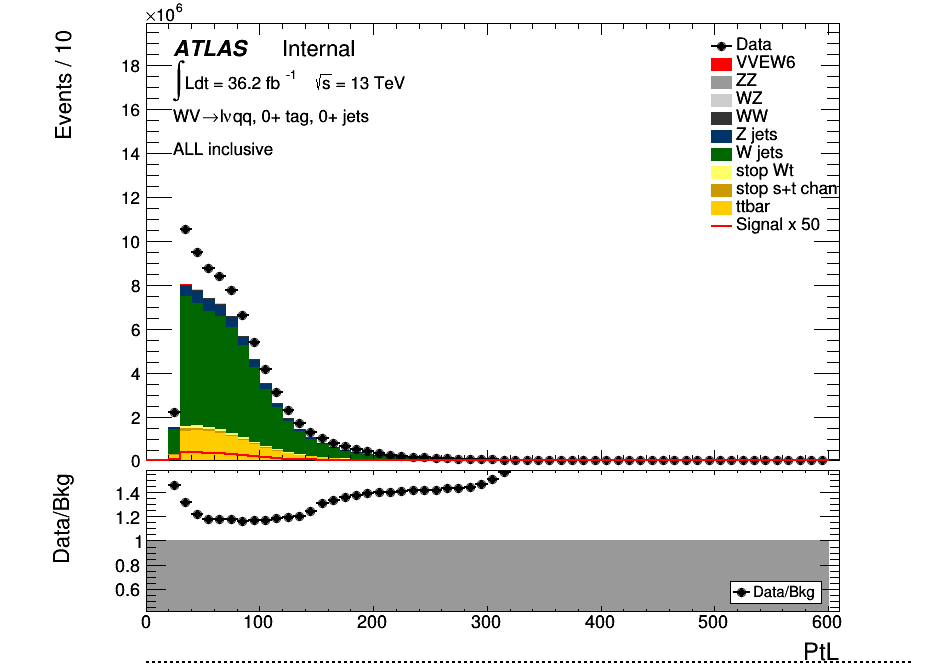
\includegraphics[width=\linewidth]{figures/1lep/CRPlots/C_0ptag0pjet_0ptv_ALL_PtL_Lin.png}
            \caption{$p_{T,l}$ before any event selection.}
        \end{subfigure}
        \begin{subfigure}{0.3\textwidth}
            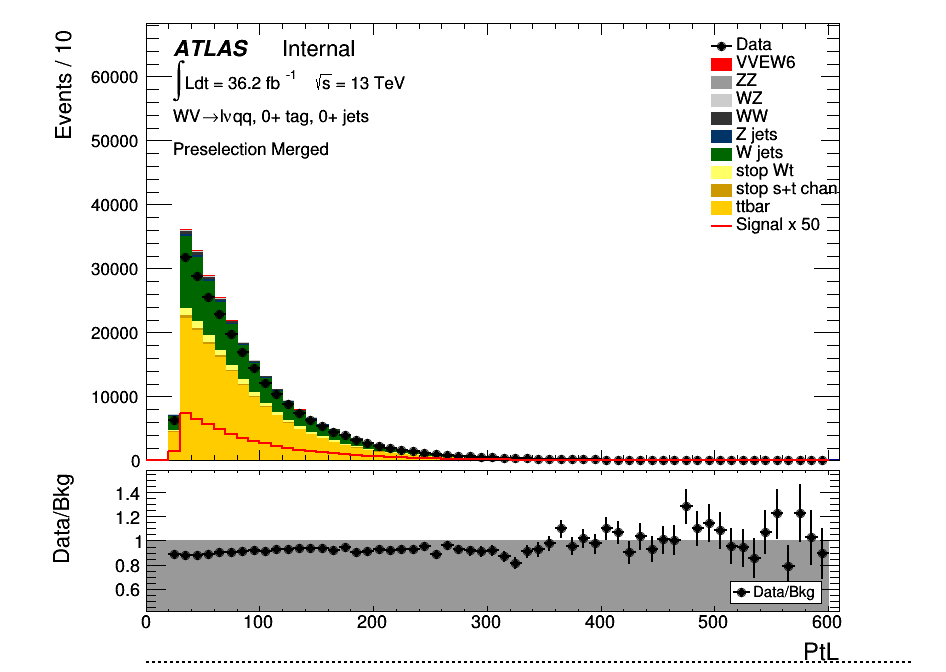
\includegraphics[width=\linewidth]{figures/1lep/CRPlots/C_0ptag0pjet_0ptv_Presel_Merged_PtL_Lin.png}
            \caption{$p_{T,l}$ after merged common preselection.}
        \end{subfigure}
        \begin{subfigure}{0.3\textwidth}
            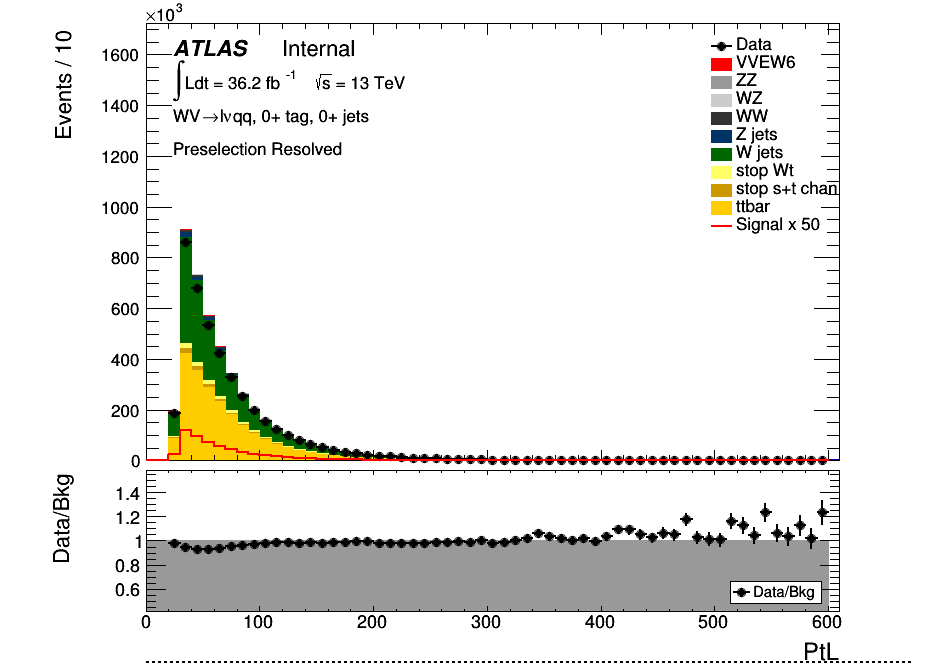
\includegraphics[width=\linewidth]{figures/1lep/CRPlots/C_0ptag0pjet_0ptv_Presel_Resolved_PtL_Lin.png}
            \caption{$p_{T,l}$ distribution after common resolved preselection.}
        \end{subfigure} \\

        \begin{subfigure}{0.3\textwidth}
            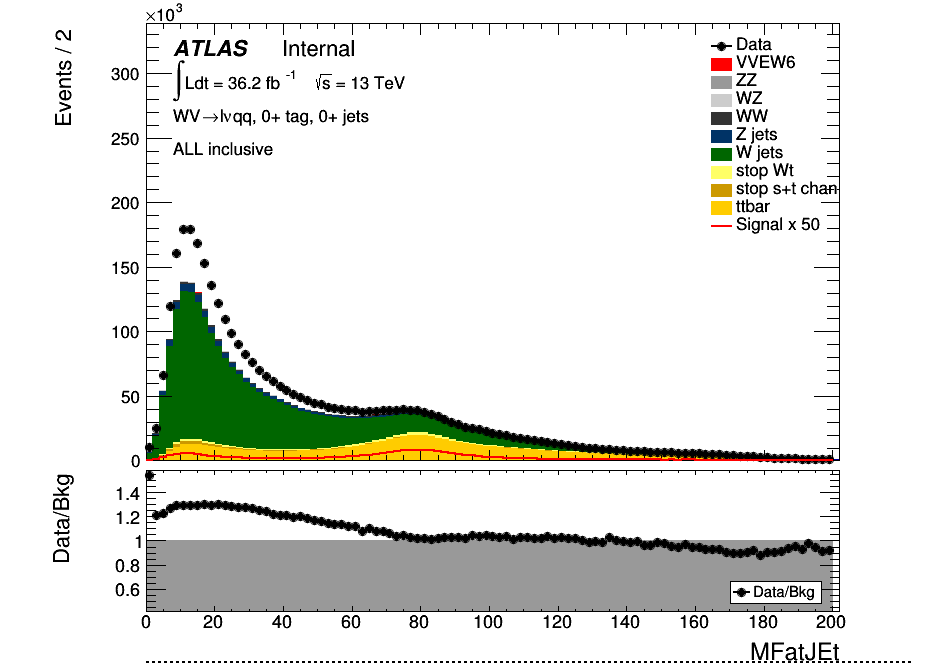
\includegraphics[width=\linewidth]{figures/1lep/CRPlots/C_0ptag0pjet_0ptv_ALL_MFatJet_Lin.png}
            \caption{$M_{J}$ before any event selection.}
        \end{subfigure}
        \begin{subfigure}{0.3\textwidth}
            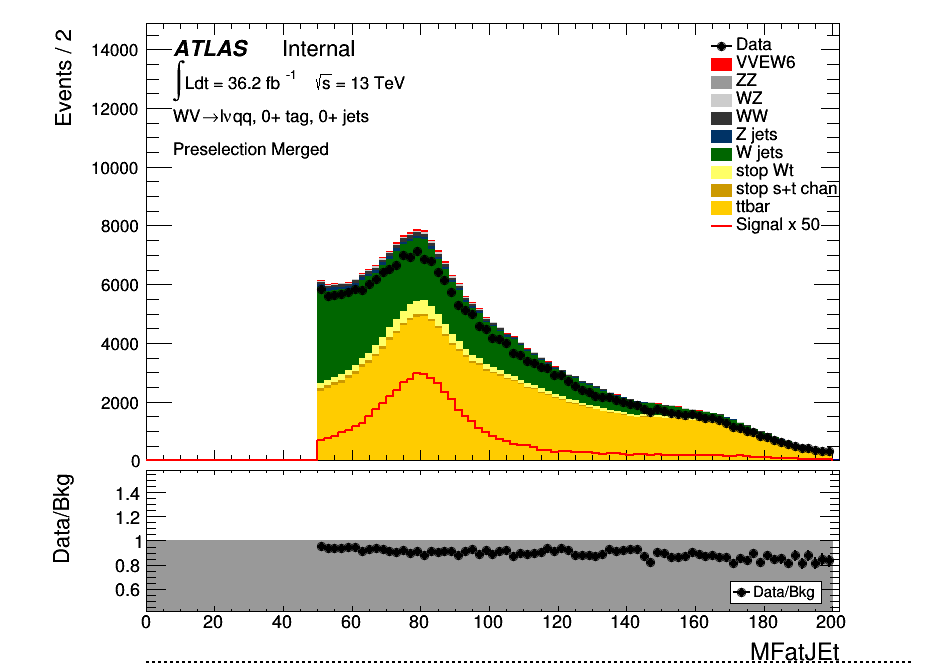
\includegraphics[width=\linewidth]{figures/1lep/CRPlots/C_0ptag0pjet_0ptv_Presel_Merged_MFatJet_Lin.png}
            \caption{$M_{J}$ after merged common preselection.}
        \end{subfigure}

        \caption{Distributions for $E_{T,miss}$, $E_{T,miss}$, and $m_{J}$ in the 1 lepton channel at different stages of the analysis selection; preselection merged and preslection resolved labels refers to the set of cuts applied in the merged and resolved regime rather than the boson tagger cuts (merged) and the signal jets mass window cut.}
        \label{fig:1LepPreselCuts}
\end{figure}


%%%\begin{figure}[ht]
%%%\centering
%%%	\subfigure[$E_{T,miss}$ before any event selection.]{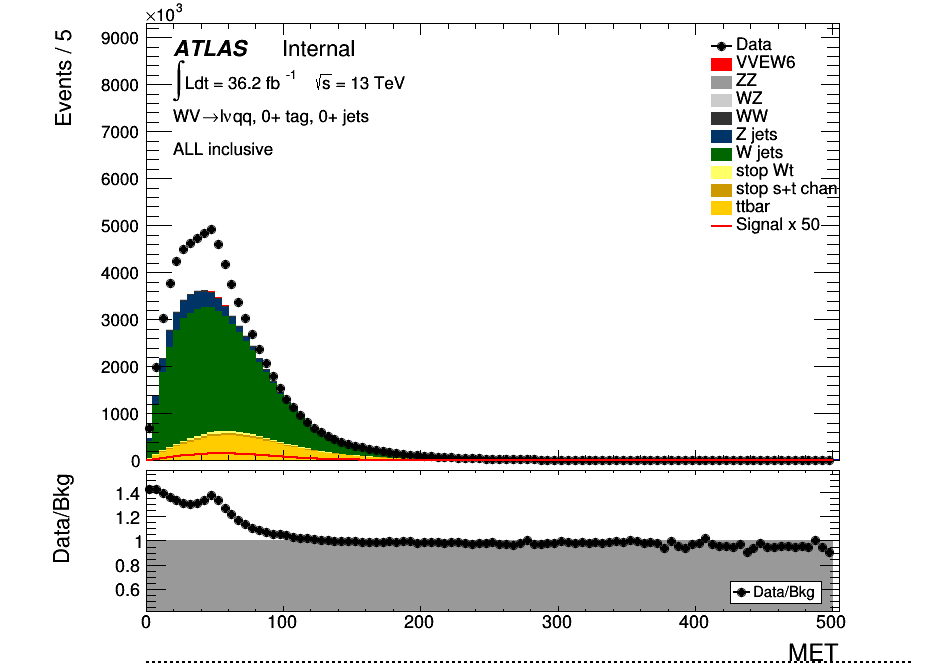
\includegraphics[width=0.3\textwidth]{figures/1lep/CRPlots/C_0ptag0pjet_0ptv_ALL_MET_Lin.png}} 
%%%	\subfigure[$E_{T,miss}$ after merged common preselection.]{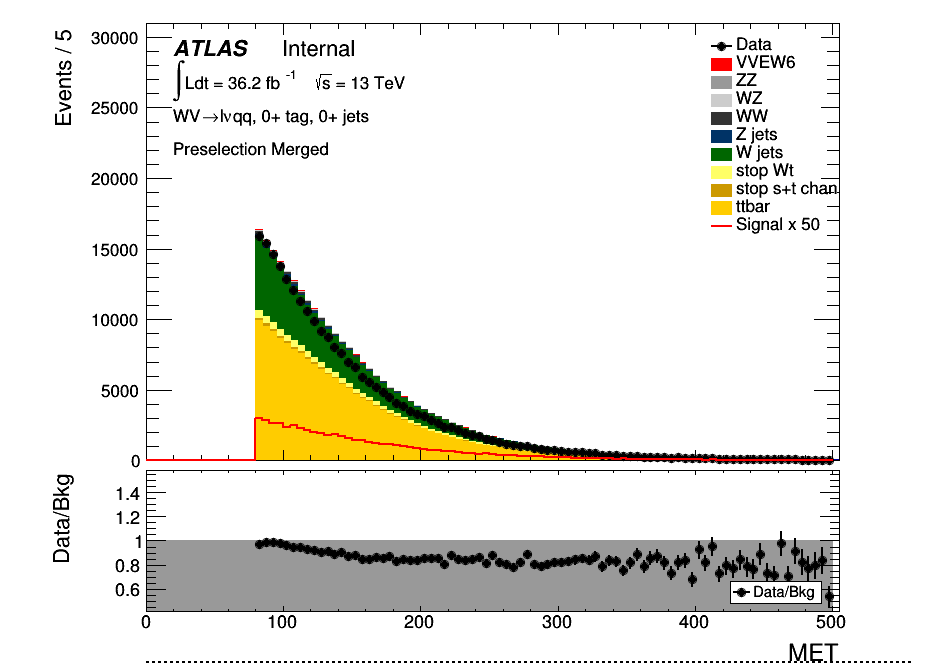
\includegraphics[width=0.3\textwidth]{figures/1lep/CRPlots/C_0ptag0pjet_0ptv_Presel_Merged_MET_Lin.png}} 
%%%	\subfigure[$E_{T,miss}$ distribution after resolved common preselection.]{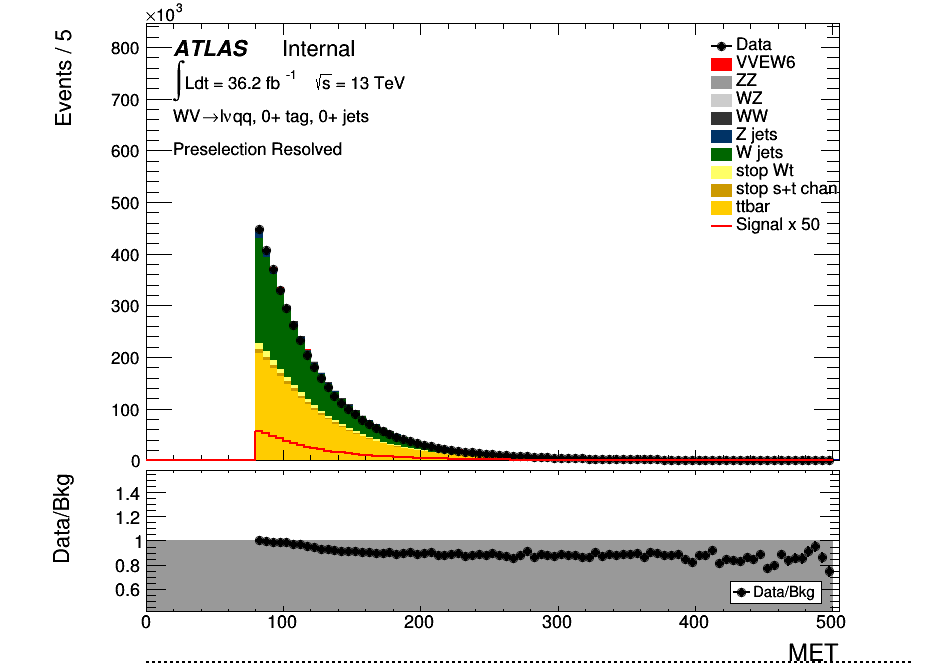
\includegraphics[width=0.3\textwidth]{figures/1lep/CRPlots/C_0ptag0pjet_0ptv_Presel_Resolved_MET_Lin.png}} \\
%%%
%%%	\subfigure[$p_{T,l}$ before any event selection.]{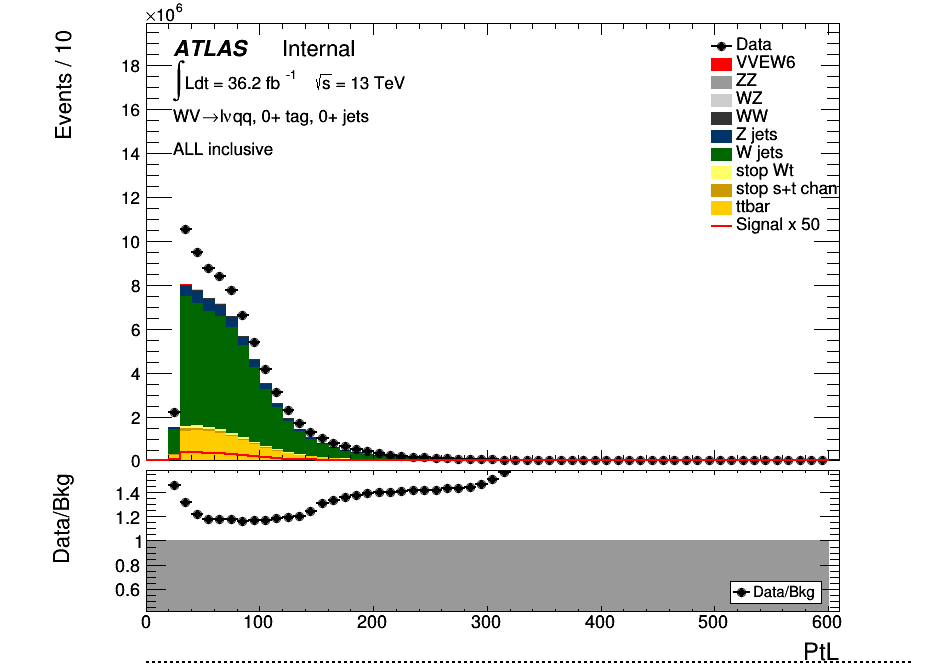
\includegraphics[width=0.3\textwidth]{figures/1lep/CRPlots/C_0ptag0pjet_0ptv_ALL_PtL_Lin.png}} 
%%%	\subfigure[$p_{T,l}$ after merged common preselection.]{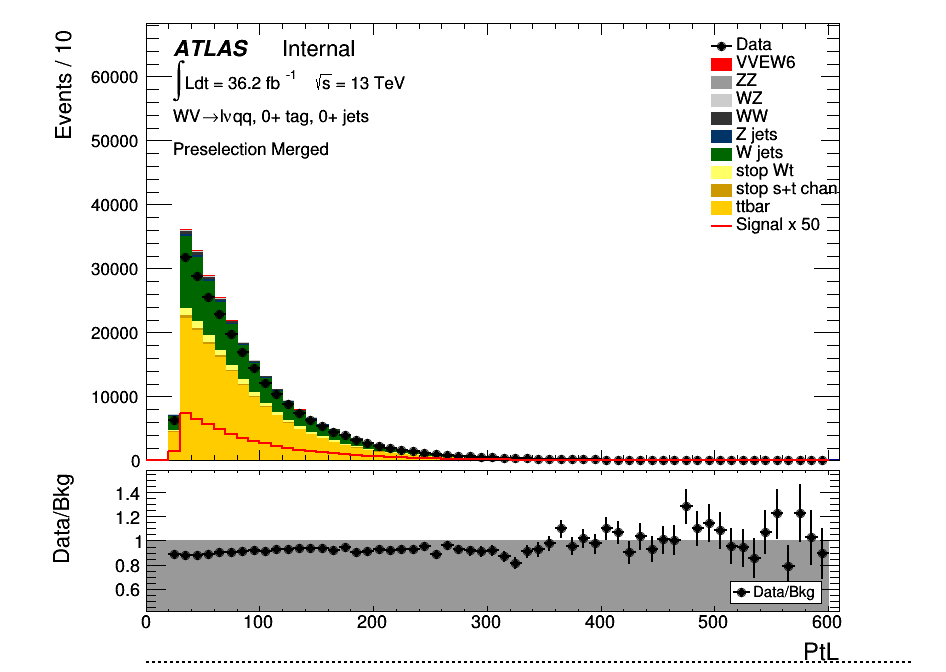
\includegraphics[width=0.3\textwidth]{figures/1lep/CRPlots/C_0ptag0pjet_0ptv_Presel_Merged_PtL_Lin.png}} 
%%%	\subfigure[$p_{T,l}$ distribution after common resolved preselection.]{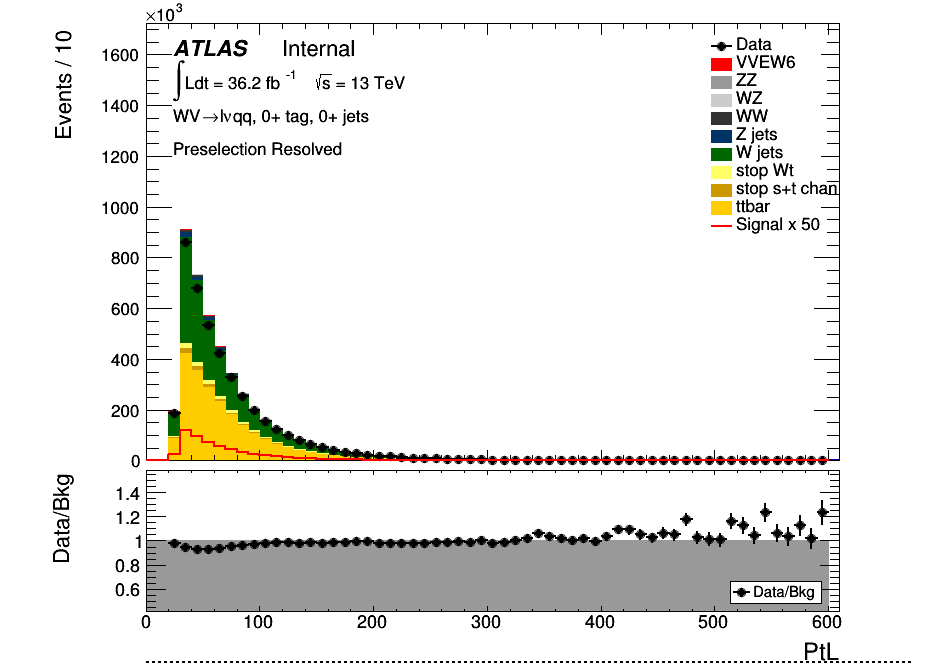
\includegraphics[width=0.3\textwidth]{figures/1lep/CRPlots/C_0ptag0pjet_0ptv_Presel_Resolved_PtL_Lin.png}} \\
%%%
%%%	\subfigure[$M_{J}$ before any event selection.]{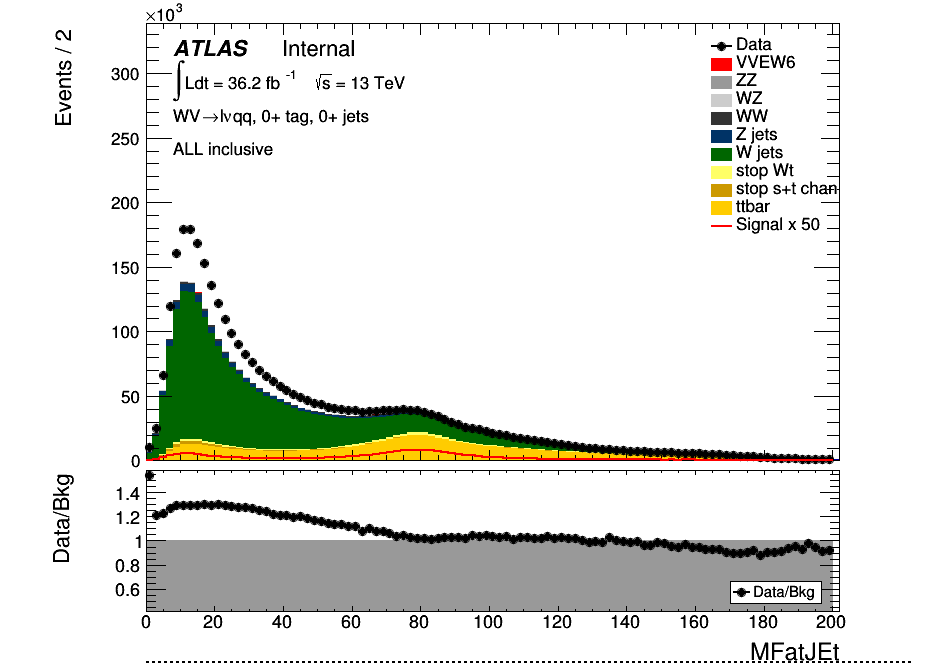
\includegraphics[width=0.3\textwidth]{figures/1lep/CRPlots/C_0ptag0pjet_0ptv_ALL_MFatJet_Lin.png}} 
%%%	\subfigure[$M_{J}$ after merged common preselection.]{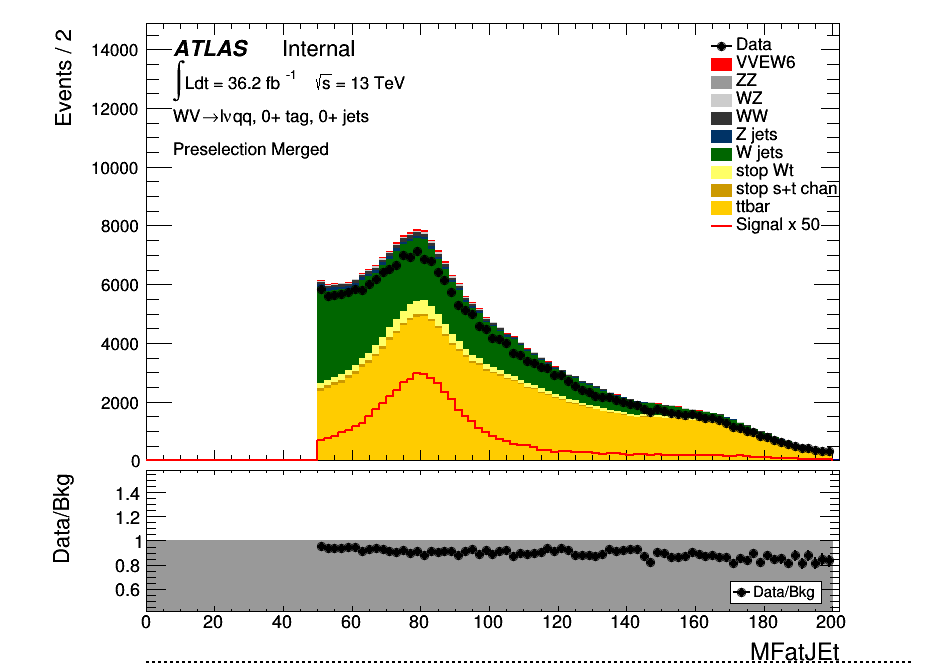
\includegraphics[width=0.3\textwidth]{figures/1lep/CRPlots/C_0ptag0pjet_0ptv_Presel_Merged_MFatJet_Lin.png}} 
%%%
%%%	\caption{Distributions for $E_{T,miss}$, $E_{T,miss}$, and $m_{J}$ in the 1 lepton channel at different stages of the analysis selection; preselection merged and preslection resolved labels refers to the set of cuts applied in the merged and resolved regime rather than the boson tagger cuts (merged) and the signal jets mass window cut.}
%%%	\label{fig:1LepPreselCuts}
%%%\end{figure}


%After the $W \to \ell\nu$ selection above and $W/Z \to jj$ selection described in Section~\ref{subsubsec:resolved_jets_selection},
%the following selection cuts are required to take the event topology of which two high-\pt\ bosons are back--to--back in the $x$--$y$ plane:
%\begin{itemize}
%\item $\Delta \phi(\ell, \met)< XX$;
%\item $\Delta \phi(j1,j2) < XX$;
%\item $\Delta \phi(\ell,j1(2)) > XX$;
%\item $\Delta \phi(j1(2), \met) > XX$;
%\end{itemize}
%where $\Delta \phi(i, j)$ is the distance in the  coordinate between objects $i$ and $j$.

%%% 2-leptons channel

%In particular, modelling of the leading and sub-leading muon \pt look slighlty different. 
%This is an effect of the first bin in both distributions that has different values in the 
%data/MC ratio. After removing the first bin in the subleading muon \pt distribution the modelling
%qfor the two muons \pt is consistent as checked in Appendix \ref{app:leptonin2lep}.

